%%%%%%%%%%%%%%%%%%%%%%%%%%%%%%%%%%%%%%%%%
% Simple Sectioned Essay Template
% LaTeX Template
%
% This template has been downloaded from:
% http://www.latextemplates.com
%
% Note:
% The \lipsum[#] commands throughout this template generate dummy text
% to fill the template out. These commands should all be removed when 
% writing essay content.
%
%%%%%%%%%%%%%%%%%%%%%%%%%%%%%%%%%%%%%%%%%

%----------------------------------------------------------------------------------------
%	PACKAGES AND OTHER DOCUMENT CONFIGURATIONS
%----------------------------------------------------------------------------------------

\documentclass[12pt]{article} % Default font size is 12pt, it can be changed here



\usepackage[labelfont=bf]{caption}

\usepackage{geometry} % Required to change the page size to A4
\geometry{a4paper} % Set the page size to be A4 as opposed to the default US Letter

\usepackage{graphicx} % Required for including pictures
\graphicspath{ {.} }

\usepackage{float} % Allows putting an [H] in \begin{figure} to specify the exact location of the figure
\usepackage{wrapfig} % Allows in-line images such as the example fish picture
\usepackage{url}

\usepackage{lipsum} % Used for inserting dummy 'Lorem ipsum' text into the template

\linespread{1.5} % Line spacing

\setlength\parindent{0pt} % Uncomment to remove all indentation from paragraphs

\graphicspath{{Pictures/}} % Specifies the directory where pictures are stored
\usepackage[left, modulo, pagewise]{lineno}


%in the preamble
%--------------------------------
\usepackage[utf8]{inputenc}
\usepackage[english]{babel}
 
 
 %Import the natbib package and sets a bibliography  and citation styles
\usepackage{natbib}
\bibliographystyle{plainnat}
\setcitestyle{authoryear,open={(},close={)}}

\usepackage{titlesec}
\newcommand{\sectionbreak}{\clearpage}


%--------------------------------


\begin{document}

%----------------------------------------------------------------------------------------
%	TITLE PAGE
%----------------------------------------------------------------------------------------

\begin{titlepage}
\title{Assignment 4}
\newcommand{\HRule}{\rule{\linewidth}{0.5mm}} % Defines a new command for the horizontal lines, change thickness here


\center % Center everything on the page

\textsc{\LARGE University Tübingen}\\[1.5cm] % Name of your university/college
\textsc{\Large Autophagy and Longevity}\\[0.5cm] % Major heading such as course name
%\textsc{\large CIS610S}\\[0.5cm] % Minor heading such as course title
\textsc{\large Essay}\\[0.5cm]

\HRule \\[0.5cm]
 \huge \bfseries The role of autophagy-regulator  mTORC1 for longevity\\ % Title of your document
\HRule \\[0.5 cm]



\begin{minipage}{0.4\textwidth}
\begin{center} \large
%\emph{Author:}\\
Sean Klein% Your name
\end{center}
\end{minipage}
\\[4cm]

{\large July 27, 2020}\\[3cm] % Date, change the \today to a set date if you want to be precise ... July 2020

%\includegraphics{Logo}\\[1cm] % Include a department/university logo - this will require the graphicx package

\vfill % Fill the rest of the page with whitespace

\end{titlepage}

%----------------------------------------------------------------------------------------
%	TABLE OF CONTENTS
%----------------------------------------------------------------------------------------

\tableofcontents % Include a table of contents

\newpage % Begins the essay on a new page instead of on the same page as the table of contents 

%----------------------------------------------------------------------------------------
%	INTRODUCTION
%----------------------------------------------------------------------------------------

\begin{linenumbers*}
\linenumbers
\section{Introduction} % Major section

\subsection{Autophagy} Autophagy is a cellular recycling process for degradation of various types of cytosolic material. It is evolutionary conserved and can be found in all eukaryotes. The mechanism as a whole is crucial for cell survival, as it is used to dispose of potentially dangerous molecules inside the cell, a common example for such molecules are aggregated proteins which have lost their functionality. These molecules will be broken down in order to be reused for cellular functions \citep{Mercer2018}.

The term of autophagy refers to multiple different processes sharing the same goal, which is cellular clearance. The predominant form is called macroautophagy (referred to as autophagy in this essay) and refers to the degradation via an so called autophagosome. These organelles' main purpose is to provide nutrients for vital cellular functions, but serves the selective elimination of unwanted or dangerous cytosolic material as well.
After induction via PI3P, which is produced by autophagic phosphoinositide 3-kinase (PI3K), a substructure on the endoplasmic reticulum (ER) is formed. From this so called omegasome a second sickle-shaped structure, the double-membraned phagophore, is created and eventually separated from the ER. Through continuous elongation of the phagophoral membrane, the vesicle eventually sequesters its degradable cargo, creating the autophagosome. Afterwards, the autophagosome fuses with the lysosome, forming the autolysosome. This enables the autophagosomal cargo to come in contact with the lysosomal lumen, leading to its degradation \citep{RabanalRuiz2018, Mercer2018, Dikic2018}. 
The process of autophagy either occurs constructively or induced by one or multiple stress signals. In both cases, autophagy is either targeting functionally redundant or damaged intracellular structures or the generation of required nutrients. The inducing stress signals can range from various nutrient deprivations, growth factor depletion, infection, hypoxia, protein aggregation, ER-stress to oxidative stress.
Other mechanisms of autophagy include microautophagy and chaperone-mediated autophagy, where the cellular material is directly transported to the lysosome \citep{Shafei2017}. 

\subsection{mTOR} The mammalian or mechanistic target of rapamycin (mTOR) serine-threonine kinase serves as a master-regulator of autophagy by coordinating cell growth and cell division in response to energy and nutrient levels as well as growth signals. 
mTOR forms two different mutliprotein signalling complexes. The mTOR Complex 1 (mTORC1) contains, in addition to mTOR, the regulatory-associated protein of mammalian target of rapamycin (Raptor), mammalian lethal with Sec13 protein 8 (mLST8), the two inhibitory subunits proline-rich Akt substrate of 40 kDa (PRAS40) and DEP domain containing mTOR-interacting protein (DEPTOR). While mTORC2 also contains mTOR, mLST8 and DEPTOR, it also consists of rapamycin-insensitive companion of mTOR (Rictor) and the regulatory subunits Sin1 and Protor 1/2 instead of Raptor. As the names of the subunits imply, both complexes differ in their sensitivity to rapamycin, which acts as an inhibitor. mTORC1 plays an important role in the regulation of cell growth via the induction and repression of anabolic and catabolic processes respectively. Therefore, one of the main functions of mTORC1 is the inhibition of autophagy. On the other hand, mTORC2 is involved in survival, architecture, polarity, growth and proliferation of the cell, but  it's role for autophagy is only minor, because of which mTORC1 will be the main focus of this essay
\citep{RabanalRuiz2018, Sciarretta2018}. Deregulation of mTOR is associated with different diseases such as diabetes, different types of cancers and neurodegenerative diseases and also ageing \citep{RabanalRuiz2018, Sciarretta2018}.

\subsection{Intention}

In this essay I want to give an overview about the current knowledge on mTORC1 and it's regulation as well as the effects mTORC1 activity has on longevity. Furthermore, I would like to discuss possible uses for mTORC1 regulation as treatment for different diseases as a way of improving life expectancy, but also want to consider the possible downsides an intervention in the regulation of mTORC1 might bring.

\section{The mTORC1 pathway}

\subsection{The Role of Rheb and it's localisation} The subcellular position of mTORC1 varies with it's activity and thus the state of autophagy activation. 
Evidence suggests that the localisation of mTORC1 towards the lysosome (or the vacuole in yeast) is required for its activation leading to the inhibition of autophagy.
This has partly to do with the small GTPase Ras-homologue enriched in brain (Rheb). This enzyme is irremovable from the lysosomal membrane but also vital for activation of mTORC1. This regulatory mechanism is controlled in a double-directional manner, as the binding of GTP not only results in Rheb activating mTORC1 (Fig. \ref{prot}), but the GDP-bound form of Rheb can also inhibit mTORC1 \citep{Noda2017, Carroll2017}. 
It is to be noted that Rheb itself is regulated by the tuberous sclerosis complexes 1 \& 2 (TSC1/TSC2).
This pair of protein complexes is capable to prevent activation of mTORC1 by Rheb resulting in the inhibition of autophagy, whose exact function and regulation will be discussed later \citep{RabanalRuiz2017}.

\begin{figure}
\centering
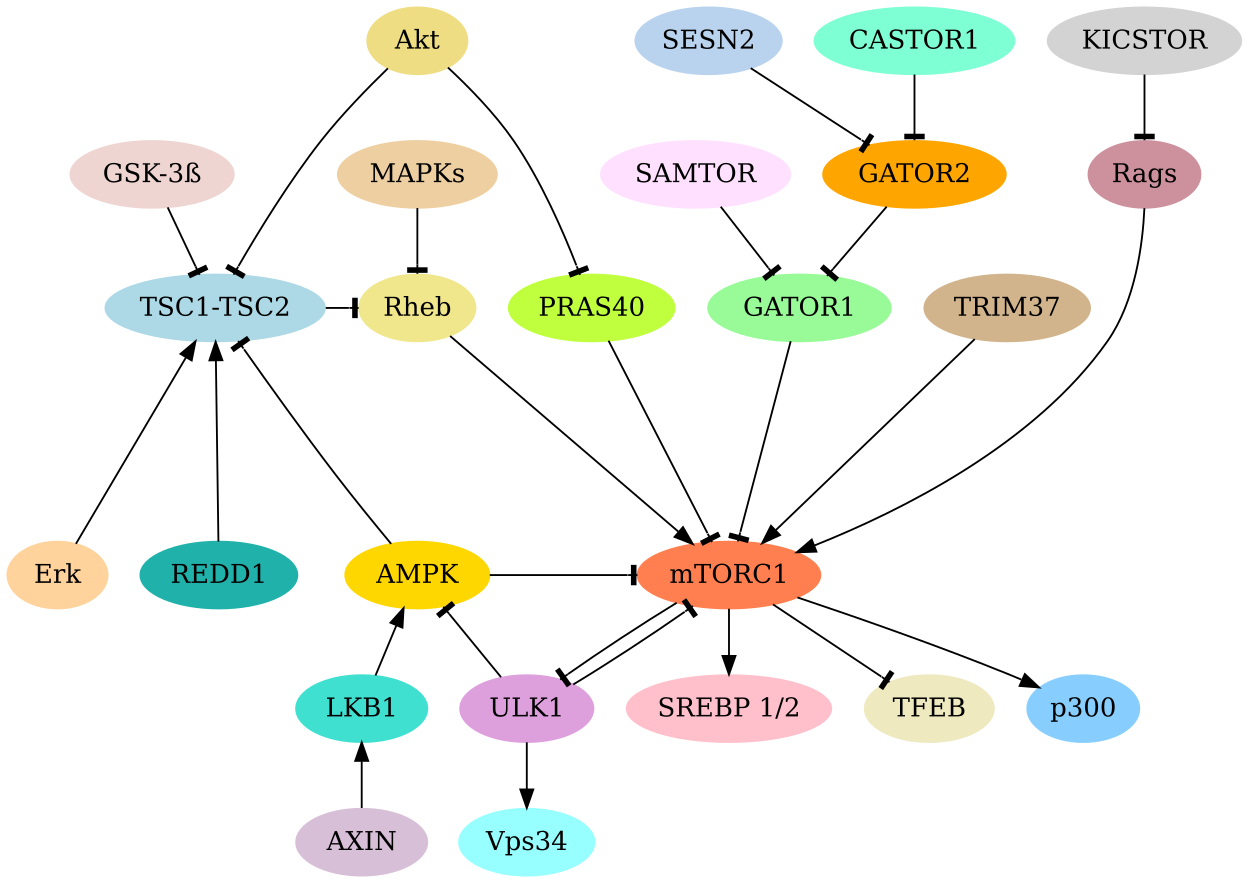
\includegraphics[width=\textwidth]{proteins}
\caption{\textbf{Role of autophagy-related proteins and protein complexes in their respective active state. Shown are the various proteins interacting directly or indirectly with mTORC1.} As by convention, each arrow represents an activating or inhibiting interaction. However, in order to maintain a good overview, protein complexes were simplified and shown as single molecules. For each such case, the node is named after their eponymous subunit.} 
\label{prot}
\end{figure}

\newpage
\subsection{Interaction with ULK1}
The main initiator for Autophagy is the unc-51-like autophagy activating kinase 1 (ULK1) complex, which is directly regulated by mTORC1 (Fig. \ref{prot}). It consists of four subunits, which are the ULK1 itself, the autophagy related proteins (ATG) 13 and 101 as well as the scaffold protein focal adhesion kinase family interacting protein of 200 kDa (FIP200)  \citep{Mercer2018, Sciarretta2018}. 
This complex induces phagophore nucleation, which is followed by the initiation of autophagosome formation. This interaction also requires the WD-repeat domain phosphoinositide-interacting proteins (WIPI) to be present. Each of the four WIPI proteins known to exist in mammalian cells are important for different aspects of phagophore formation \citep{Dikic2018, Mercer2018}. 
Under nutrient-rich conditions, mTORC1 binds and phosphorylates the subunits ULK1 and ATG13 in order to deactivate the ULK1 Complex.  Meanwhile under low energy levels (depletion of ATP), the AMP-activated protein kinase (AMPK) becomes active and phosphorylates ULK1 (Fig. \ref{prot}) in a manner different to mTORC1, resulting in the activation of autophagy instead. Interestingly, ULK1 inhibits AMPK and mTORC1 by phosphorylation, resulting in an triangular relationship between these complexes. %positive and negative feedback loop at the same time?
\citep{Mercer2018, Sciarretta2018, RabanalRuiz2018}
The downstream target of ULK1 is the class III phosphoinositide 3-kinase Vps34 (Fig. \ref{prot}). It's complex consists of VPS34, beclin 1 (BECN1), and the pseudokinase p150 (PIK3R4) and either ATG14 or UV radiation resistance-associated gene protein (UVRAG). Wile the ATG14-bound version of the complex is involved in autophagosome nucleation, the UVRAG-bound complex regulates later stages of autophagy. The former is again inhibited by mTORC1 in it's active form, hindering its function as the initiator of autophagy %maybe add something about PI3P?
\citep{Mercer2018, RabanalRuiz2018}.
The mTORC1 complex also plays a role in the creation of autophagosomes apart from its interaction with ULK1. The transcription factor EB (TFEB) controls cellular clearance but is inhibited by mTORC1 (Fig. \ref{prot}). Only under starvation conditions TFEB activity is able to regulate gene expression of genes involved in lysosomal biogenesis and lipid catabolism \citep{Dikic2018}. The tripartite motif containing 37 (TRIM37) also is an important factor in the interaction between mTORC1 and TFEB, where TRIM37 helps with the activation of mTORC1 (Fig. \ref{prot}) as well as allowing TFEB to be phosphorylated by mTORC1 \citep{Wan2018}.
Interestingly, it was recently shown that TFEB also meditates endocytosis and that this process plays an important role in the reactivation of mTORC1 during starvation \citep{Nnah2019}.

\subsection{Rag GTPases}
Just as Rheb, the Rag GTPases are also members of the Ras superfamily and are another important sensor for nutrient availability. The four different Rag proteins form heterodimers. Therefore, either Rag A or Rag B form a complex with Rag C or Rag D. In order to reach an active state to enable them to localise on the lysosomal membrane, Rag A/B has to bind GTP while Rag C/D has to bind GDP. This allows mTORC1 to to bind to the Rag-dimer via Raptor and promote it's activation and localisation to the lysosome (Fig. \ref{prot}). Changing the conformation where Rag A or B bind GDP and Rag C or D bind GTP inactivates the complex and releases mTORC1 from the lysosome. 
\citep{RabanalRuiz2018, Carroll2017}.
Rag plays an important role in the sensing of amino acids. One example is Sestrin 2 (SESN2), which acts as a leucine sensor. During amino acid deprivation, it deactivates GAP activity toward Rags 2 (GATOR2), which otherwise would positively regulate mTORC1 . GATOR2 does this by binding and disabling GATOR1. The KICSTOR-Complex binds and recruits GATOR1 to the lysosome where it acts as an inhibitor of the Rag GTPases as seen in figure \ref{prot} \citep{Gu2017}.  
Other proteins are PAT1 and the cellular arginine sensor for mTORC1 (CASTOR1). Because of its involvement in the transport of alanine, glycine and proline, PAT1 is suspected to meditate the amino acid-dependent regulation of mTORC1 localisation (Fig. \ref{prot}). Meanwhile, CASTOR1 impacts the GATOR1/2 pathway in response to low arginine levels inside the cell
\citep{RabanalRuiz2018, Shafei2017, Sciarretta2018}.

Since the Rag heterodimer cannot bind the lysosome on their own, the Ragulator complex is required for linkage to the lysosome. The Ragulator complex consists of five lysosomal adaptor and MTOR activator (LAMTOR) proteins. If associated with the Rag GTPases, the Ragulator-Rag Complex also interacts with the vacuolar-type H\textsuperscript{+}-ATPase (v-ATPase), which is a multimeric proton pump. Again, this protein fulfills multiple roles in the process of autophagy. First, its function as a proton pump is responsible for creating the acidic environment inside the lysosome necessary for later degradation of autophagosomal cargo. Secondly, the v-ATPase plays a role in AMPK-dependent autophagy induction, which will be discussed later.
Due to their role for the localisation of mTORC1 to the lysosomal Surface, Ragulator and the Rag proteins are crucial for activation of mTORC1 by Rheb.


\subsection{TSC complexes}
One major Regulator of Rheb are the tuberous sclerosis complexes 1 and 2 (TSC1 and TSC2), which themselves form the TSC1-TSC2 complex. The main role of this complex is the inhibition of Rheb activity (Fig. \ref{prot}). Because of the inhibition, Rheb is unable to hydrolyze GTP into GDP. The GTP-bound Rheb permits mTORC1 to localise to the lysosome and thus inhibit autophagy
\citep{Dikic2018}.
Although seeming basic, the role TSC plays in autophagy becomes clear on inspection of its interactome. TSC2 is a prominent target for phosphorylation in order to hinder it's function and to promote autophagy. As shown in figure  \ref{prot} the regulators of the TSC complexes are numerous. They include Protein kinase B (Akt) in presence of growth factors, the AMP-activated protein kinase (AMPK) in response to energy or glucose deprivation, the extracellular-signal-regulated kinase (Erk) and  glycogen synthase-3$\beta$ (GSK-3$\beta$), again during energy depletion \citep{RabanalRuiz2017}. Apart from the TSC-complexes, Rheb is also directly inhibited by p38 mitogen-activated kinases (MAPKs) during energy deprivation as well \citep{Sciarretta2018}.

TSC is also involved in the growth factor signalling pathway. The scarcity of growth factors mediates the activation of via PI3K/Akt which leads to the inhibition of TSC2 by phosphorylation via Akt (Fig. \ref{prot}). This results in the dissociation from lysosome and allowing the activation of mTORC1  \citep{Dikic2018}. TSC2 inhibits Rheb at same time. Coincidentally, Akt also inhibits the mTORC1 subunit PRAS40. This stops the inhibition of Raptor by PRAS40, therefore strengthening the activation of mTORC1 as seen in figure \ref{prot} \citep{RabanalRuiz2018}.
The TSC2 complex is also regulated by the interaction of FIP200 and WD-repeat domain phosphoinositide-interacting protein (WIPI) 3, which represents a link between regulation of autophagy and autophagosome formation \citep{Dikic2018}.
One other positive regulator is the hypoxia-induced stress protein REDD1 (regulated in development and DNA damage responses 1), which activates the TSC1-TSC2 complex independent of AMPK \citep{Dikic2018, RabanalRuiz2018}.
Specific growth factor stimuli activate the extracellular signal–regulated kinases (ERKs) 1 and 2, which also has been shown to activate mTORC1 via phosphorylation-based inhibition of TSC2 \citep{Huang2008}.
To summarize, the TSC complexes are involved in many different forms of stress-induced regulation of autophagy, such us intracellular energy levels, cytokines, or hypoxia.
TSC2 complex is also strongly regulated by the availability of amino acids. in the case of amino acid scarcity, the TSC2 complex has been shown to be lysosomally localised. This Influence even nullifies growth factor signalling. Therefore both, amino acids and growth factor signalling, are required to maintain the cytoplasmic localisation of TSC2
\citep{RabanalRuiz2018}. 

% The importance of amino acids for autophagy will be discussed later. Also discussed later in more detail, these processes are often regulated be specific amino acids. In consequence it has been demonstrated that arginine is capable tof relieving the allosteric inhibition of Rheb by the TSC complex already mentioned above \citep{RabanalRuiz2018}.


\subsection{Interaction with AMPK}
Another previously mentioned protein complex is AMPK. It acts antagonistic towards mTORC1 and thus plays a similarly important role in the process of autophagy. It is activated in response to an allosteric binding of AMP, representing low energy levels, or during glucose deprivation, which results in inhibiting biogenic synthesis in order to allow the cellular energy stores to be restocked \citep{Huang2008, RabanalRuiz2018}.
As a major positive regulator of autophagy, the inhibition of mTORC1 is ensured in two ways. First, AMPK directly inhibits mTORC1 by phosphorylating the raptor subunit and secondly by phosphorylating TSC2 as already mentioned (Fig. \ref{prot}). Both of these interactions lead to the lysosomal dissociation and thereby inactivation of mTORC1.
\citep{RabanalRuiz2017, Mercer2018, Carroll2017}.
Another Interaction of AMPK with relation to autophagy is the activation of ULK1 by phosphorylation . This is an interesting way in which AMPK is able to bypass mTORC1 in order to induce autophagy. However, ULK1 also phosphorylates all three AMPK subunits to down-regulate AMPK activity during starvation . The result is an interesting negative feedback-loop (Fig. \ref{prot}), which prevents over-activation of autophagy \citep{Mercer2018, Carroll2017}.
AMPK is activated by liver kinase B1 (LKB1) which is meditated by AXIN either in presence of AMP or upon glucose  (Fig. \ref{prot}).
During this activation the AXIN/LKB1-AMPK complex binds to the Ragulator subunit LAMTOR1 (Late Endosomal/Lysosomal Adaptor, MAPK And MTOR Activator), which strictly requires the previously mentioned v-ATPase to be present. AXIN itself is also involved in the starvation-induced dissociation and thereby inactivation of mTORC1 \citep{RabanalRuiz2018, Shafei2017, Carroll2017}.
In addition to that, AXIN mediates the activation of AMPK by serine/threonine-protein kinase STK11 (LKB1) upon glucose starvation or in presence of AMP \citep{Dikic2018, Carroll2017}.
Interestingly, low cellular ATP levels lead to the impairment of protein folding as well as ER stress. Both events are known to help with the activation of autophagy \citep{RabanalRuiz2018}.

\subsection{Nutrient-dependent activation of mTORC1}
As autophagy is activated when the cell is starving certain nutrients, consequently, mTORC1 activity is increased when the cell has enough nutrients. %is mTORC1 activity increased dependent on the amount of nutrients missing? if only one AA is missing the others might get overproduced??
One of the most important nutrients relevant for autophagy control are amino acids
\citep{Carroll2017}. 
It has to be noted however, that different amino acids may impact the deactivation of autophagy in different ways. One deciding factor might be whether the amino acid, the cell is missing, is an essential one or not. The dealing with different amino acids can be observed on the molecular level, which will be the topic of the following paragraph.
\cite{Carroll2017} summarized, that leucine, arginine and glutamine are the main amino acids that drive mTORC1 activation. All of them are considered essential, at least under certain conditions, some form of stress for example, which might also trigger autophagy
\citep{Reeds2000, Fuerst2004}.
During glutaminolysis, a process in which glutamine is synthesized, $\alpha$-ketoglutarate ($\alpha$-KG) is created as an intermediate. It has been shown that $\alpha$-KG induces the activation of mTORC1 \citep{Carroll2017, RabanalRuiz2018}.
Interestingly, this process is supported by leucine availability due to it being required as a cofactor for one of the enzymes involved in glutaminolysis. The sensing of leucine happens via SESN2, which binds the amino acid resulting in an activation of mTORC1 due to the release of SESN2  from GATOR2 allowing the inhibitory interaction with GATOR1 to take place \citep{Carroll2017, RabanalRuiz2018}.
The sensing of arginine is quite similar to that of leucine. Here, the amino acid binds to CASTOR1, which in turn prevents the interaction of CASTOR1 with GATOR2, allowing inhibition of GATOR1 by GATOR2 (Fig. \ref{prot}). As a result mTORC1 can be activated by the Rag GTPases leading to an increase in mTORC1 signalling \citep{Carroll2017,Carroll2016,RabanalRuiz2018}.
Another amino acids identified to play a role in autophagy is methionine. This essential amino acid is sensed by the SAMTOR, which is interacting with GATOR1 to hinder mTORC1 signaling. More precisely, the presence of S-adenosyl methionine (SAM) disrupts the binding to and inhibition of GATOR1 \citep{Gu2017}.
Despite the importance individual amino acids might have, none is sufficient for activation of mTORC1 in cell, that still starve other amino acids important for autophagy regulation \citep{Noda2017}.
It has also been shown that rapamycin, which is an important molecule due to its pharmacological implications for the activation of autophagy, can circumvent the effects that amino acids have and activate the degradative despite their presence by interaction with mTORC1 \citep{Noda2017}.

\subsection{Involvement outside of autophagy}
\paragraph{Involvement in translation} 
Translation is one of the most fundamental processes present in almost all cells independent of organism. The mTORC1 complex represents the connection between autophagy and the regulation of translation. This relation makes sense, since one of the main objective of autophagy is the removal of proteins from the cell, which then might be required to be reproduced. Therefore mTORC1 is able to activate ribosomal protein S6 kinase beta-1 (S6K1). This protein then promotes the initiation of translation via various mechanisms as well as preventing PDCD4 (programmed cell death 4), which also results in an increase of translation \citep{Sciarretta2018}.

\paragraph{Control over transcription}
The mTORC1 complex also impacts other cellular processes by regulation of transcription. The complex can activate the transcription factor sterol-responsive element-binding protein 1/2 (SREBP 1/2) (Fig. \ref{prot}) which induces the expression of genes involved in fatty acid metabolism, cholesterol biosynthesis and the oxidative pentose pathway. The role mTORC1 plays does not seem to be minor though, as the activation of SREBP 1/2 happens via multiple different ways, directly and indirectly \citep{Sciarretta2018}. Other regulations of gene expression include positive regulation of the nucleotide synthesis promoting activating transcription factor 4 (ATF4); the enhancement of the expression of multiple genes involved in mitochondrial biogenesis, which makes sense in the scenario where mTORC1 is reactivated after the degradation of mitochondria via selective autophagy (mitophagy); as well as the enhancement of expression of hypoxia-inducible factor-1$\alpha$ (HIF-1$\alpha$), this induces a metabolic shift from fatty acid oxidation towards glycolysis \citep{Sciarretta2018}.
Histone acetyltransferase (HAT) p300 is another case fitting the picture. Activation of p300 by mTORC1 (Fig. \ref{prot}) results in the upregulation of lipogenesis, but also the inhibition of autophagy. This is another case where mTORC1 represents the molecular connection between two logically connected cellular processes \citep{Wan2017}.

\subsection{Outlook}
Although the aspects mentioned above are very introductory and no explanation is by any means exhaustive, it might not have become clear how much is still unknown. While a lot of the fundamental mechanisms have been identified by now, there still could be unknown factors with the potential of having a substantial impact on the regulation of autophagy. An example for this is a lysosome-localized G protein-coupled receptor like protein (GPR137B). It only has been found in 2019 to control the localization of Rag and mTORC1 \citep{Gan2019}. Hence, we do not know how many other proteins are yet to be discovered and what role they might play in process of autophagy.

%write something about solute carrier family if necessary (carrol and RabanalRuiz2018) and about v-ATPase (noda2017)
%TODO: look for info on other amino acids or other nutrients outside of Carroll2017

% in Summary: activation of mTORC1 requires two conditions:
% translocation of the complex to the lysosomal surface (stimulated by nutrients and Rag GTPases)
% activation by GTP-bound Rheb (regulated by cellular signalling cascades and the availability of energy, 
% and oxygen and different nutrients than the ones for Rags)
%Autophagy is an important avenue for nutrient supply, particularly during amino acid starvation which contributes amino acids to restore mTORC1 activity
%In turn, autophagy-mediated restoration of mTORC1 induces autophagy termination and reformation to lysosomes which complete the feedback loop

\section{Implications of mTORC1 control for longevity}

\subsection{The connection between longevity and diseases}
%something about no natural cause of death at high ages
Generally autophagy has the potential to help with treatment and prevention of many diseases and thus impact the life expectancy. However, the effectiveness can vary between different diseases to the point that autophagy can be counterproductive in certain cases as will be shown here on.
There are multiple categories of diseases where autophagy is or might be effective but there are also some smaller or more specific cases where autophagy has been proven to be effective. One such example is the removal of intracellular bacteria during infection \citep{Dikic2018}.
Not directly related to diseases and comparable new is the knowledge about the connections between aging and cellular senescence in general as well as it's connection to mTORC1. Therefore the mechanisms of a cell for becoming senescent can be used to limit the negative effects that can occur during ageing. It now was revealed that mTORC1 can be used as a target for elimination of such cells, creating space for new cells to grow and thus increasing the overall life expectancy \citep{Kucheryavenko2019}.
Another relatively recent discovery is the role of autophagy and mTORC1 in denervated muscles, which can be caused by of several muscle diseases. In those cases however, a tight control of mTORC1 seems necessary to allow proper healing of the affected tissue. For example a sustained activation of mTORC1 resulted in the hindrance of synaptic remodeling after such denervation events \citep{Castets2019}. Whether or not an inhibition of mTORC1 can be exploited in some non-harmful way does not seem to be entirely clear yet. 
Another case, where autophagy is already induced as a reaction automatically, is hyperammonemia. This disease describes the accumulation of ammonia in the blood stream, resulting damages can range form irreversible neuronal damage and coma to death. Comparable to the use of autophagy during neurodegenerative diseases, hepatic autophagy is facilitated to help out where other strategies of waste nitrogen removal fail to be sufficient. Here, by the inhibition of mTORC1. Additionally, an increase of autophagy seems to preventive effects, hence the inhibition of mTORC1 appears to be a potential therapy for patients with high risks of developing such conditions \citep{Soria2018}.
As will be shown later, increased autophagy via deregulation of mTORC1 does not help in preventing or fighting diseases in every case One such example is the development of metabolic diseases like type 2 diabetes following the loss of mTORC1 function in $\beta$-cells found in the pancreas \citep{BlandinoRosano2017}.

%Autophagy as cancer therapy has up- and downsides for defeating cancer >> risky
%Autophagy universally helps fighting neurodegenerative diseases
%proautohpagy drugs have shown to limit infection and inflammation


\subsection{Involvement of Autophagy in circadian rhythm}
One mechanism which does not show its relation with autophagy directly, is the circadian clock found in many eukaryotes. For mammalians it is controlled in the suprachiasmatic nucleus (SCN) by so-called "clock genes", which are  linked to mTORC1 and thereby autophagy. The circadian clock also has an impact on longevity as well as connections with autophagy as will be discussed here on.
Therefore, the histone deacetylase Sirtuin 1, encoded by the silent mating type information regulation 2 homologue 1 (Saccharomyces cerevisiae) (SIRT1) gene, is involved in the circadian-rhythm and connected to the mTOR complex as well as AMPK. This nicotinamide adenine dinucleotide (NAD\textsuperscript{+}) dependent protein controls transcription of different genes via modifications of the DNA-histones. It has been shown that SIRT1 leads to an inhibition of mTORC1 and thus promotes autophagy. Furthermore, the SIRT1 activity is increased in conjunction with AMPK. The direct connection to two major regulators of autophagy underlines the importance of the circadian clock for autophagy and vice versa
\citep{Maiese2017}.
SIRT1 is involved in multiple disease processes including cancer, vascular disease, diabetes, and neurodegenerative disorders. Many of these processes require the modulation
of autophagy by SIRT1 \citep{Maiese2017}.
The hormone melatonin, which controls the circadian rhythm, has been shown to also rely on autophagy pathways, including mTOR signalling, in order to control processes of aging and neurodegeneration 
\citep{Maiese2017}.
The control of autophagy by the circadian rhythm has multiple implications for different diseases and thereby for longevity. Multiple diseases are linked to to changes in the activity or expression of different clock genes. For example, Alzheimer is connected to a changed rhythmic methylation of Brain and Muscle ARNT-Like 1 (BMAL1), which may contribute to cognitive loss and behavior changes. Meanwhile, Parkinson patients show decreased levels of BMAL1 as well as nuclear receptor ROR-alpha (ROR$\alpha$) and some forms of cancer show an increased expression of the circadian rhythm gene TIMELESS. 
It also has been shown that circadian rhythm dysfunction during cognitive loss and aging induces autophagy to remove neural aggregates causing aging which would lead to behaviour impairments otherwise. 
Autophagy is  depressed during the absence of the PER1, a protein acting as a circadian oscillator, indicating that autophagy regulation relies on the circadian clock and changes over the course of the day
\citep{Maiese2017}.

\subsection{Cancer}

The usage of autophagy as a treatment to cancer can have downsides and will only pose as case-dependent solution. This goes to the extent that it has been referred to as a "double-edged sword" due the damage autophagy can do to cancer patients \citep{Dikic2018}.
First of all,  only some types of cancer rely on autophagy for it's survival. Therefore, an inhibition of autophagy might show no effect. However, in some cancer types, autophagy is facilitated to help to sustain the rapid growth and other behaviours specific to cancer cells, by providing the additional nutrients required. One example for such a behaviour is the oncogene polo like kinase 1 (PLK1). This commonly used tumour marker inhibits mTORC1 to active autophagy in order drive cellular proliferation helping the cancer to develop \citep{Ruf2017}.
On the other hand, the activation of autophagy could even lead to an enhanced cell death.
Hence, an inhibition might not hinder the malfunctioning cells but rather help them survive. Autophagy would have been beneficial by clearing the cell of oncogenic proteins and other damaged cellular particles that otherwise facilitate growth of the tumour \citep{Lane2017b, White2012}.
Another aspect is the impact autophagy has on the development itself.  While autophagy is believed to help to prevent tumorigenesis, it also helps the cell to survive certain conditions like inflammation, which can promote the development of cancer \citep{Lane2017b, Dikic2018}.


\subsection{Neureodegeneration}

The development of neurodegenerative diseases has shown to be influenced by the activity of autophagy. For example, the most common cause of death in animals with autophagy defects \citep{Dikic2018}. Thanks to the fact, that many of those neuron-affecting diseases are results of aggregated, misfolded or unfolded proteins, the induction of autophagy is often a good treatment strategy. These defective proteins accumulate inside neuronal cells were they would normally be degraded by proteasomes. However, if the proteasome activity fails to match the speed at which these defective proteins occur, autophagy can step in to help with clearing up the cell. Unlike the proteasomal degradation, autophagy also allows the removal of cellular organelles, which have received irreparable damage due the disease \citep{Dikic2018}. Therefore, these diseases become more severe if autophagy does not function correctly.
The ubiquitin-binding protein p62 or Sequestosome-1 has shown to be a good marker in neurodegenerative diseases. This protein is normally involved in the clearance of protein aggregates by targeting certain autophagic cargo \citep{Dikic2018, Rusten2010}.
Another cause of neurodegeneration are dysfunctional mitochondria by causing an increase in radical oxygen species. They can be removed by selective autophagy too, which is referred to as mitophagy \citep{Dikic2018}.

%\paragraph{Infection and inflammation}
%Autophagy is also involved in the removal of intracellular bacteria as well as of inflammatory agents \citep{Dikic2018}.

\subsection{The cardiovascular system}
mTORC1 and mTORC2 are crucial regulators for cardiac homeostasis, cardiac adaptation to stress and embryonic development. During development, the mTOR complexes are essential for the preservation of cardiac structure, growth, and vascular integrity. Supporting this, it has been shown that mTORC1 activation during chronic stress has multiple maladaptive effects, including the promotion of pathological hypertrophy, obviously an increase in misfolded protein accumulation and the occurrence of energy stress \citep{Sciarretta2018}.
However, an inappropriate disruption of mTORC1 can lead to undesirable consequences as well. Disruption of mTORC1 during postnatal stages of development can lead to a lack of production of fundamental proteins within cardiomyocytes. Despite the downsides it has been shown that a non-complete or moderate inhibition of mTORC1 is overall beneficial for the heart for the process of aging \citep{Sciarretta2018}.
One specific heart-related disease where mTORC1 is an important factor, is cardiac hypertrophy. The protein complex is required in its active form to compensate for cardiac hypertrophy, for maintenance of cardiac function and for the response of pressure overload. Hence autophagy is one of the cells main tools to actively and passively combat hypertrophy and activation of mTORC1 happens in response to hypertrophic signals. Despite that, it seems that mTORC1 has more of a preventive function for cardiac hypertrophy as it's activation alone does fully counteract hypertrophy \citep{Sciarretta2018}. 
An interesting aspect of hypertrophy is the responding epigenetic regulation. Thus, the inhibition of class I histone deacetylases (HDACs) suppresses pathological cardiac hypertrophy. In addition, mTORC1 targets a long non-coding RNA with the name of cardiac hypertrophy-associated epigenetic regulator. Its inactivation also reduces pathological cardiac hypertrophy and improves heart function in response to pressure overload \citep{Sciarretta2018}.
The next interesting regulation of mTORC1 observed during cardiac hypertrophy comes in form of multiple microRNAs. The RNAs miR-211 and miR-199a both seem to play a role in activation of mTOR, the significance of the latter is unclear though \citep{Sciarretta2018}.
There are other cardiovascular disorders and diseases where mTOR plays a role, but to summarize the key message, the inhibition of mTORC1 exerts beneficial effects during cardiac stress, which outweigh the downsides. It is to be noted however that mTORC2 has a more important role to prevent damage of the heart and associated cells during stress and thus should be kept active during treatment \citep{Sciarretta2018}.


%----------------------------------------------------------------------------------------
%	CONCLUSION
%----------------------------------------------------------------------------------------

\section{Conclusion} % Major section

%\subsection{Possible Treatment using autophagy and mTORC1}
There are different ways to induce autophagy in order to harvest the benefits of the cellular clean for longevity and personal health. One way would be caloric restriction in one's diets. Accordingly, caloric restriction was shown to improve diastolic function, reduce mTORC1 activity, and stimulate autophagy \citep{Sciarretta2018}.
The activation of autophagy can also be induced pharmacologically, where mTOR is only one of the potential target with already-mentioned rapamycin as the most important inducer of autophagy. This interaction is mediated via FK506-binding protein of 12 kDa–rapamycin complex (FKBP12), which binds rapamycin and then directly inhibits mTORC1 \citep{Sciarretta2018, Dikic2018}. By this way, autophagy can reduce age-related heart inflammation and fibrosis and improve the overall energy metabolism \citep{Sciarretta2018}. Interestingly, it has been found out recently that the tumor protein translationally-controlled 1 (TPT1/TCTP), which is an activator of autophagy in general, can help to further enhance the effect that rapamycin has on the induction of autophagy \citep{Bae2017}.
Nonetheless, there can be side effect of rapamycin treatment which might impact other cellular pathways in humans \citep{Dikic2018}.

Another aspect of treatment with rapamycin or it's modified analogs, so called "rapalogs", is the question what autophagy activation actually means for disease-affected cells. Since autophagy only clears the cell of damaged cellular contents, often it can not pose as the cure to the disease. This becomes apparent when looking at some diseases on more detail. In the example of cancer, the damage done to the cell is normally irreversible and the only solution is to induce cell-death in one way or another. However, the treatment with rapalogs will not be able to do this on its own since it acts cytostatic rather than cytotoxic, meaning that only the growth of cancer is hindered and the treatment would have to continue indefinitely to prevent further spreading of the tumour \citep{Lane2017b}. Although mTORC1 can be used in the elimination of senescent cells at least in vitro, this is also means that tumorigenesis has already been prevented as cellular senescence is a tumour suppressor mechanism \citep{Kucheryavenko2019}. 
Therefore these mechanisms might not be usable in cells that already developed oncogenic characteristics. 
\paragraph{} A similar case can be made for neurodegenerative diseases. Assuming the cause also an intrinsic one, it is unlikely to be resolved after a full clean-up of the damaged contents of the cells. If for example the proteasomal activity can not recover, it has to be fully replaced by autophagy. The fact that constant autophagic activity is not ideal, becomes especially prevalent in regards to the previously discussed topics. Logically, the use of constantly active autophagy can eventually lead the development of cancer. One way to reduce that risk, might be to induce autophagy only locally where it is needed. That way, non-diseased cells would be less involved so that their normal functioning could be maintained as much as possible.

It also should be noted that rapamycin is not the only viable activator of autophagy. For example, a recent investigation identified the cysteine-reactive acrylamide EN6 as another potential drug to regulate mTORC1. Since this molecule is interacting with v-ATPase, instead of directly targeting mTORC1, this could mean that treatment could result in less or different side effects. However, not enough is known yet to give a clear answer to the question whether EN6 has potential to outperform rapamycin \citep{Chung2019}.

Of course there are other applications where autophagy can in fact act as the single way to cure the cell. One example is the aforementioned infection with parasitic bacteria, which invade the cell. Because the cause can be regarded as extrinsic, clearing all of the intracellular bacteria can return the cell to a healthy state where programmed cell-death wont be necessary.

Another possibility of reducing side effects might be to target one of the many regulators upstream of mTORC1. Most of these molecules are responsible for autophagy regulation only under specific conditions. By circumventing only certain regulators of mTORC1, normal function of autophagy control could be maintained in other cases.

To summarize, the induction of autophagy has the potential to be part of a successful therapy for numerous diseases, all of which can result in an increase in longevity. Achieving this effect by an inhibition of mTORC1 seems to be promising for multiple reasons. Despite that, it has to be remembered that autophagy often is able to only fulfill a assisting role in the cure of lifespan-related diseases and should be carefully evaluated before considering the use as a treatment.

\end{linenumbers*}

%----------------------------------------------------------------------------------------
%	BIBLIOGRAPHY
%----------------------------------------------------------------------------------------


%Where the bibliography will be printed
 
\bibliography{Autophagy}

%----------------------------------------------------------------------------------------

\end{document}